%\usepackage{dtklogos}
\usetikzlibrary{mindmap,shadows}
\renewcommand{\href}[2]{#2}
% Information boxes
\newcommand*{\info}[4][16.3]{%
  \node [ annotation, #3, scale=0.65, text width = #1em,
          inner sep = 2mm ] at (#2) {%
  \list{$\bullet$}{\topsep=0pt\itemsep=0pt\parsep=0pt
    \parskip=0pt\labelwidth=8pt\leftmargin=8pt
    \itemindent=0pt\labelsep=2pt}%
    #4
  \endlist
  };
}
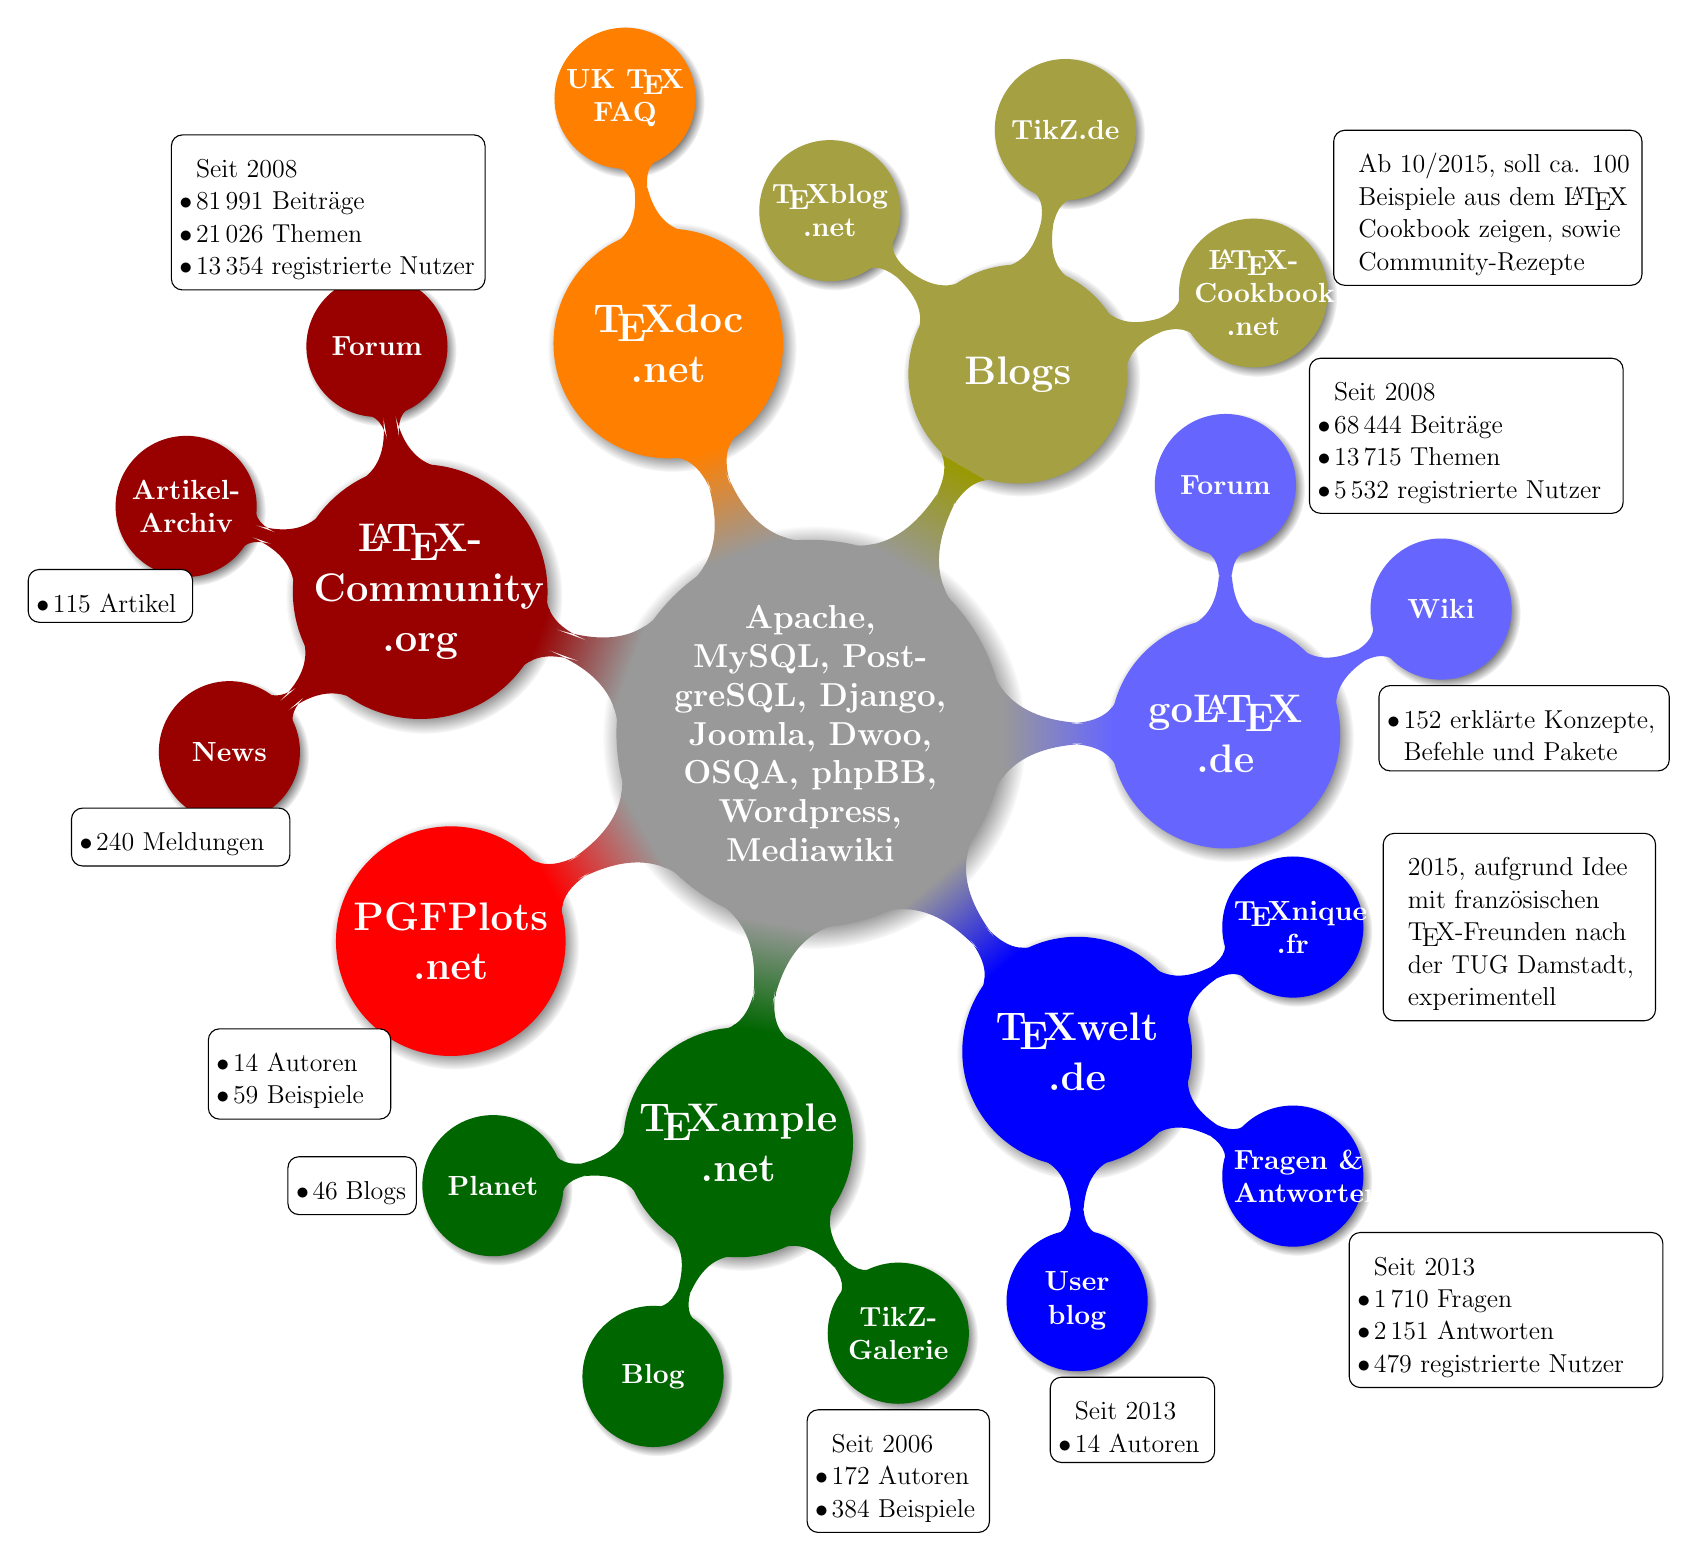
\begin{tikzpicture}[ every annotation/.style = {draw,
                     fill = white, font = \Large}]
  \path[mindmap,concept color=black!40,text=white,
    every node/.style={concept,circular drop shadow},
    root/.style    = {concept color=black!40,
      font=\large\bfseries,text width=10em},
    level 1 concept/.append style={font=\Large\bfseries,
      sibling angle=50,text width=7.7em,
    level distance=15em,inner sep=0pt},
    level 2 concept/.append style={font=\bfseries,level distance=9em},
  ]
  node[root] {Apache, MySQL, PostgreSQL, Django, Joomla,
    Dwoo, OSQA, phpBB, Wordpress, Mediawiki} [clockwise from=0]
    child[concept color=blue!60] {
      node {\href{http://golatex.de}{go\LaTeX\\.de}} [clockwise from=90]
        child { node (goForum) {\href{http://golatex.de/index.html}{Forum}} }
        child { node (goWiki) {\href{http://golatex.de/wiki/Hauptseite}{Wiki}} }
    }
    child[concept color=blue] {
      node[concept] {\href{http://texwelt.de}{\TeX welt\\.de}}
        [clockwise from=30]
      child { node[concept] (TeXnique)
        {\href{http://texnique.fr}{\TeX nique\\.fr}} }
      child { node[concept] (TeXweltQA)
        {\href{http://texwelt.de/wissen/}{Fragen~\& Antworten}} }
      child { node[concept] (TeXweltBlog)
        {\href{http://texwelt.de/blog/}{User blog} }}
    }
    child[concept color=green!40!black] {
      node[concept] {\href{http://texample.net/}{\TeX ample\\.net}}
        [clockwise from=310]
      child { node[concept] (TikZGalerie) 
        {\href{http://texample.net/tikz/examples/}{TikZ-Galerie}} }
      child { node[concept] (TeXampleBlog)
        {\href{http://texample.net/weblog/}{Blog}} }
      child { node[concept] (Planet)
        {\href{http://texample.net/community/}{Planet}} }
    }
    child[concept color=red] {
      node[concept] (PGFPlots) {\href{http://pgfplots.net}{PGFPlots\\.net}}
      [clockwise from=270]
    }
    child[concept color=red!60!black] {
      node[concept] {\href{http://latex-community.org/}{\LaTeX-Community\\.org}}
        [counterclockwise from=100]
      child { node[concept] (LaTeXForum)
        {\href{http://latex-community.org/forum/}{Forum}}}
      child { node[concept] (LaTeXArtikel)
        {\href{http://latex-community.org/know-how}{Artikel-Archiv}} }
      child { node[concept] (LaTeXNews)
        {\href{http://latex-community.org/home/news}{News}} }
    }
    child[concept color=orange] {
      node[concept] (TeXdoc)
        {\href{http://texdoc.net/}{\TeX doc\\.net}}
        [clockwise from=100]
        child { node[concept] {\href{http://www.tex.ac.uk}{UK \TeX \\FAQ}}
        }}
    child[concept color=yellow!60!black] {
      node[concept] (Blogs) {Blogs} [clockwise from=139]
      child { node[concept] {\href{http://texblog.net/}{\TeX blog\\.net}}}
      child { node[concept] {\href{http://tikz.de/}{TikZ.de}} }
      child { node[concept] (Cookbook)
        {\href{http://latex-cookbook.net/}{\LaTeX-\\Cookbook\\.net}} }
    };
    \info{goForum.north east}{above,anchor=west,xshift=1em}{%
      \item[] Seit 2008
      \item 68\,444 Beiträge
      \item 13\,715 Themen
      \item 5\,532 registrierte Nutzer
    }
    \info{LaTeXForum.north west}{above,anchor=south}{%
      \item[] Seit 2008
      \item 81\,991 Beiträge
      \item 21\,026 Themen
      \item 13\,354 registrierte Nutzer
    }
    \info[8]{LaTeXArtikel.west}{below,anchor=north east,xshift=3em,yshift=-2em}{%
      \item 115 Artikel
    }
    \info[11]{LaTeXNews.south west}{below,anchor=north}{%
      \item 240 Meldungen
    }
    \info[9]{TikZGalerie.south}{below,anchor=north}{%
      \item[] Seit 2006
      \item 172 Autoren
      \item 384 Beispiele
    }
    \info[15]{goWiki.south}{below,anchor=north,xshift=3em}{%
      \item 152 erklärte Konzepte, Befehle und Pakete
    }
    \info{TeXweltQA.south east}{above,anchor=north west}{%
      \item[] Seit 2013
      \item 1\,710 Fragen
      \item 2\,151 Antworten
      \item 479 registrierte Nutzer
    }
    \info[8]{TeXweltBlog.south}{below,anchor=north,xshift=2em}{%
      \item[] Seit 2013
      \item 14 Autoren
    }
    \info[9]{PGFPlots.south west}{anchor=north east,xshift=1em}{%
      \item 14 Autoren
      \item 59 Beispiele
    }
    \info[6]{Planet.west}{anchor=east}{%
      \item 46 Blogs
    }
    \info[14]{TeXnique.east}{anchor=west,xshift = 0.5em}{%
      \item[] 2015, aufgrund Idee mit französischen
              \TeX-Freunden nach der TUG Damstadt, experimentell
    }
    \info[16]{Cookbook.east}{anchor=south west}{%
      \item[] Ab 10/2015, soll ca. 100 Beispiele aus
              dem \LaTeX\ Cookbook zeigen, sowie
              Community-Rezepte
    }
\end{tikzpicture}
